% \documentclass[journal, 12pt, onecolumn, draftclsnofoot]{IEEEtran} %JSAC 20'
\documentclass[sigconf]{acmart} %ACM Mobihoc 20'
\usepackage[linesnumbered,vlined,ruled]{algorithm2e}
\usepackage{algorithmic}
\usepackage{amsmath,amsthm,amssymb,amsfonts}
\usepackage{color}
\usepackage{dcolumn}
\usepackage{graphicx}
\usepackage[utf8]{inputenc}
\usepackage{soul}
\usepackage{mathtools}
\graphicspath{ {./images/} }
%---------------------------------------------------------------%
\newtheorem{definition}{Definition}
\theoremstyle{definition}
\newtheorem{program}{Program}
\newtheorem{assumption}{Assumption}
\newtheorem{example}{Example}
\newtheorem{Algorithm}{Algorithm}
\newtheorem{policy}{Policy}
\newtheorem{problem}{Problem}
\theoremstyle{remark}
\newtheorem{remark}{Remark}
\theoremstyle{plain}
\newtheorem{theorem}{Theorem}
\newtheorem{lemma}{Lemma}
\newtheorem{corollary}{Corollary}
%---------------------------------------------------------------%
\newcommand{\eq}{=}
\newcommand{\domZ}{\mathbb{Z}_{*}}
\newcommand{\domP}{\mathbb{Z}_{*}}
\newcommand{\vecOne}{\mathbf{1}}
\newcommand{\ind}{\mathbf{I}}
\newcommand{\mat}{\mathbf}
\newcommand{\Poisson}{\text{Poisson}}
\newcommand{\Bernoulli}{\text{Bernoulli}}
\newcommand{\define}{\triangleq}
\newcommand{\leadto}{\Rightarrow}
\newcommand{\vecG}{\boldsymbol}
\renewcommand{\vec}{\mathbf}
\DeclarePairedDelimiter{\set}{\{}{\}}
\DeclarePairedDelimiter{\norm}{|}{|}
\DeclarePairedDelimiter{\Inorm}{\|}{\|_1}
\DeclarePairedDelimiter{\Paren}{\bigg(}{\bigg)}
\DeclarePairedDelimiter{\Bracket}{\bigg[}{\bigg]}
\DeclarePairedDelimiter{\Brace}{\bigg\{}{\bigg\}}
%---------------------------------------------------------------%
\newcommand{\fixit}[1]{{\color{red}{#1}}}
\newcommand{\accept}[1]{#1}
\newcommand{\deny}[1]{\st{#1}}
\newcommand{\comments}[1]{{\color{blue}{#1}}}
\newcommand{\delete}[2]{}
\newcommand{\needref}[1]{\text{[#1]}}
%---------------------------------------------------------------%
\newcommand{\AP}{\dagger}
\newcommand{\ES}{\ddagger}
\newcommand{\apSet}{\mathcal{K}}
\newcommand{\esSet}{\mathcal{M}}
\newcommand{\ccSet}{\mathcal{X}}
\newcommand{\jSpace}{\mathcal{J}}
\newcommand{\Stat}{\mathbf{S}}
\newcommand{\Obsv}{\mathcal{Y}}
\newcommand{\Policy}{\vecG{\Omega}}
\newcommand{\Baseline}{\vecG{\Pi}}
\newcommand{\algname}{Solver}
%---------------------------------------------------------------%
\newcommand{\brlatency}{\emph{broadcast latency}}
% \newcommand{\brpoint}{\emph{broadcast point}}

%---------------------------------------------------------------%
%%
%% \BibTeX command to typeset BibTeX logo in the docs
\AtBeginDocument{%
  \providecommand\BibTeX{{%
    \normalfont B\kern-0.5em{\scshape i\kern-0.25em b}\kern-0.8em\TeX}}}

%% Rights management information.  This information is sent to you
%% when you complete the rights form.  These commands have SAMPLE
%% values in them; it is your responsibility as an author to replace
%% the commands and values with those provided to you when you
%% complete the rights form.
% \setcopyright{acmcopyright}
% \copyrightyear{2018}
% \acmYear{2018}
% \acmDOI{10.1145/1122445.1122456}
%---------------------------------------------------------------%

\begin{document}
    \title{Stale Information-based Cooperative Jobs Dispatching in Edge Computing System}

    \author{HONG Yuncong}
    % \affiliation{
    %     \institution{The University of Hong Kong}
    %     \streetaddress{Pokfulam Rd}
    %     \city{Hong Kong}
    %     \state{Hong Kong}
    %     \country{China}
    % }
    % \email{ychong@cs.hku.hk}

    \begin{abstract}
    In this paper, we consider the distributive job dispatching problem in an edge computing network residing in Metropolitan area network (MAN), where the job arrivals, uploading latency and computation time are all random.
    Specifically, multiple access points (APs) collect jobs from the mobile users, and upload each job to one edge server according to its type.
    The job arrivals, uploading latency and computation time are all random.
    APs and edge servers periodically broadcast their local state information, and the APs update their job dispatching strategy according to partially observable boradcast information.
    We formulate the optimization of job dispatching strategy as a partially observable Markov decision process (POMDP), whose minimization objective is a discount measurement of job delivery and computation delay.
    The conventional solution for POMDP is impractical due to huge complexity.
    In this paper, we propose a novel low-complexity solution framework to address the issue of algorithm complexity.
    Specifically, we first derive the analytical expression of the approximate value function according to baseline policy.
    Based on it, the optimization of job dispatching strategy can be decoupled via an alternative policy iteration algorithm, so tha the policy iteration of each AP can be made according to the partially observable system state information.

    % In this paper, we consider the cooperative job dispatching problem in an edge computing network residing in Metropolitan area network (MAN).
    % Multiple access points (APs) are deployed to collect jobs from the mobile users, and distributed make dispatching decisions on edge servers for each job.
    % The coordination in a multi-agent system (MAS) requires agents to share the same utility function via information sharing.
    % While existing literature seldomly consider the information sharing latency among multiple agents, the latency is actually not negligible in such extensive network.
    % And making decisions based on stale information may result into irremediable estimation error of the system status.

    % We address the impact of latency on future system performance, and formulate the optimization problem as an infinite horizon Markov decision process (MDP), where the randomness of job uploading, processing time is considered.
    % In this problem, the approximate MDP should be adopted to address the curse of dimensionality.
    % Conventional low-complexity approximate solution of MDP is usually hard to predict the performance analytically.
    % We then propose a novel approximate MDP solution framework via one-step policy iteration over baseline policy, where the analytical performance bound can be obtained.
    % It is shown by simulations that the proposed low-complexity algorithm can effectively reduce the \emph{average job response time} per job of the considered edge computing network.
\end{abstract}

% \ccsdesc[500]{Computer systems organization~Embedded systems}
% \ccsdesc[300]{Computer systems organization~Redundancy}
% \ccsdesc{Computer systems organization~Robotics}
% \ccsdesc[100]{Networks~Network reliability}

% \keywords{datasets, neural networks, gaze detection, text tagging}
    \maketitle

    
\section{Introduction}
Edge Computation is believed to be a promising technology for solving increasingly communication congestion in backbone network.
(Rich-media tasks are delay-sensitive).
\cite{Naha2018} is a survey about fog computing in delay-aware computing in IoT, and investigate numerous proposed computing architecture.


Related works on job dispatching on scheduling in edge computing, mostly with centralized agent to apply action and seldom take delayed information impact into consideration.
There are some previous works on jobs scheduling strategies under the scenario of edge computation, together with joint optimization job dispatching and resource allocation:
\begin{itemize}
    \item \cite{Zheng2019} is a work considering maximizing the long-term utility in MEC offloading policy, and formulating the problem with MDP solved with Q-learning (However, it's applied with a centralized controller which would suffer from communication overhead, and without performance guarantee);
    \item \cite{Du2018} propose an offline algorithm with MINLP (Mixed-Integer Nonlinear Programming) problem formulation, considering min-max fairness guarantee in computation offloading and computation resource allocation in fog/edge computing scenario (However, with only one edge and one cloud node considered);
    \item \cite{Alameddine2019} is a work considering task offloading, scheduling and resource allocation joint optimization with Benders Decomposition (However, delay information is previous defined);
    \item \cite{Fan2017} considers cooperation of multiple MEC-BSs of computation offloading to other MEC-BSs (However, it doesn't consider the offloading utility impact on other MEC-BSs, i.e. only optimize for one BSs in the cluster).
\end{itemize}


Different from the previous referred works, which only consider optimization for one agent in system or using centralized agent for decision making, we focus on the impact of out-of-dated information on decision making in multiple agents distributed cooperation.
Due to frequent jobs releasing from users and uncertainty of jobs uploading time to servers, the obsolete information is inevitable in a purely distributed system.
This information sharing delay would cause severe mis-estimate for job dispatching decision making, and thus it will be hard to guarantee the cooperation among individual agents.
Moreover, the information sharing delay is often un-deterministic due to shared under-laid network topology, and offensively sharing strategy would cause network congestion to other normal functions.


As what we have learned for now, there are very limited discussions on this topic:
\begin{itemize}
    \item The earliest works entangling with out-of-dated information we could find is \cite{ref-01} (cited 167 times). In this work, the single agent is assumed not able to observe the global state, and thus they need communication to establish cooperation by sharing limited information. The agent considers communication as extra action to synchronize the states and thus incurs extra cost (However, the communication is without delay, thus converted into POMDP problem; criticize with impractical);
    \item The other work \cite{ref-02} considers continuous state observation with constant or stochastic delay with single agent;
    \item One researcher published a series of paper on this topic \cite{Lyu2017,Lyu2018,Lyu2018a,Lyu2018b}.
        \cite{Lyu2017} is work considering \emph{partial out-of-date knowledge} optimization in IoT computing scenario, with Lyapunov optimization;
        \text{[delay-sensitive, ToC]} \cite{Lyu2018} identify that task admission is critical to delay-sensitive applications in mobile edge computing, and proposes an (1-$\epsilon$)-approximation algorithm
        \text{[foggy, fully distributed online]} \cite{Lyu2018a} is a work fully distributed online optimization to minimize the time-average cost and achieve asymptotic optimality over infinite time;
        \cite{Lyu2018b} try to establish cooperation among selfish devices in fog computing, and out-of-date information is blamed for optimality gap but proved to asymptotically diminish with the proposed algorithm (However, the out-dated information is considered with limited effect);
\end{itemize}

%NOTE: [abandon useless references]
% Service Placement Scenario:
% \begin{itemize}
%     \item \cite{Rodrigues2017} is a work on minimizing service delay in mobile edge computing;
%     \item \cite{Yang2016} is a work considering services placement and requests dispatching on edge servers, and leverage users' pattern to predict "service cache" for online decision making;
%     \item \cite{Chen2018} is a work with SDN on task offloading and battery life saving, and solve the NLP problem with two sub-problems;
% \end{itemize}
% Using Game Theory:
% \begin{itemize}
%     \item \cite{yang2018} and \cite{Josilo2019a} considers distributed computation offloading game;
%     \item \cite{Liu2018} is a work considering minimize users' power consumption with Lyapunov optimization and matching theory;
%     \item \cite{Dinh2018} considers distributed multi-user offloading in wireless channel with selfish EPG (exact potential game);
%     \item \cite{Josilo2019} considers selfish offloading to achieve Nash equilibrium;
%     \item \cite{Chen2016} is a work considering multi-user computation offloading with multi-channel contention, and adopt game theory approach to achieve Nash equilibrium with upper bound of convergence time;
%     \item \cite{Zhang2018} considers multi-user offloading under transmit power decision and user association decision;
% \end{itemize}
% System Work:
% \begin{itemize}
%     \item \cite{Yu2018} is a system work published in ToMC, presents a framework to minimize remote execution overhead, and carry out real system experiments using large-scale data from cellular network provider;
%     \item \cite{Wang2018} is a system work published in IEEE Access, considers the mobility of mobile users in limited coverage solved with service migration and handover, and propose a framework;
% \end{itemize}

In this article, we consider there are Access Points (APs) in this network to connect the mobile users and edge servers.
The computation jobs would be released from UEs and the dispatching decisions are determined distributed on each AP nodes as depicted in Fig.\ref{fig:system}.
The information sharing scheme is proposed in this article with synchronized broadcast design. With the help of this scheme, we could immediately apply the job dispatching decision based on obsolete information, with some prior stochastic knowledge of global system.
Our contributions are summarized as follows.
\begin{itemize}
    \item To our best knowledge, we are the first work to propose the MDP framework making use of obsolete information in edge computing system. With shared prior stochastic knowledge about broadcast delay and uploading delay, the distributed agent could come to consensus on optimal policy adopting globally;
    \item We propose a global state MDP formulation to characterize the multiple-agent problem, i.e. single agent would consider multiple-agent decision optimality to achieve cooperation.
    We with adopt value function approximation to reduce the traditional algorithm complexity, and come up with performance guarantee performance bound.
\end{itemize}


The remainder of this paper is organized as follows.
In Sec.II, we justify the motivation on our topic.
And then we illustrate the system model and the optimization problem formulation in Sec.III and Sec.IV respectively.
In Sec.V, we introduce a low-complexity MDP algorithm to the .
In Sec.VI, we show the results of evaluation.
In Sec.VII, the conclusion is given.
    % \input{src/02a-background}
    % \section{Motivation}
%----------------------------------------------------------------------------------------%
Nowadays, the edge computing system always presences in a distributed formation.
There are clusters of Edge Servers in cooperation but separated physically, together serve the jobs released from edge devices.
Different from classical Cloud Server scenario usually with centralized scheduler design, the cooperation among clusters encounters with problems which disturb it from centralization design, such as: reasonable cooperation mechanism, un-timely and disorder information sharing and unpredictable underlaid network condition (compared with data center network).

%NOTE: 
Firstly, an efficient information sharing scheme design is needed in such distributed system.
In edge computing scenario, we consider the clusters are of same coalition and they cooperate to achieve a global optimal target, e.g. minimum job execution time.
The local greedy policy under this situation would have no insight.
We design a periodic sampling scheme in our problem.
\begin{example}[Periodic Sampling Error]
    The periodic sampled status is already a good estimation for Job Completion Time (JCT).
\end{example}
Under the assumption of periodic information sharing, it's actually a quite practical model 

%NOTE: second point
Secondly, with intensive jobs release from edge devices, the \brlatency is the key issue to take care in dispatching decision design.
\begin{example}
    Fixed one AP, the one would adopt sub-optimal policy before receiving the information. A.k.a, sub optimal plus optimal in that period is not optimal
\end{example}
The insight exists in: the bottleneck may exist in Barrel Theory that one lacking AP could ruin the whole cooperation on the target.
And we only do delay-aware instead of delay-adapt policy.

%NOTE: third point
Last but not least, the biggest challenge in the way of distributed decision making is unpredictability of underlaid network delay.
In this article, we propose model-based reinforcement learning problem formulation, to adapt with stochastic environment.
To alleviate the curse of dimensionality, we propose a one-step value iteration approximation to solve the Bellman's Equation, which is with performance guarantee.

%NOTE: additional point
Additionally, we don't consider further offloading onto cloud infrastructure in our scheme.
For two reasons: maybe it's without performance guarantee as there's no explicit computation model for cloud; maybe edge clusters cooperation is already enough as a replacement; 


    \section{System Model}
%----------------------------------------------------------------------------------------%
\subsection{Network Model}
We consider an edge computing system with $K$ Access Points (APs) and $M$ edge servers, which are connected in a network as illustrated in Fig.\ref{fig:system}.
The sets of APs and edge servers are denoted as $\apSet \define \set{1,\dots,K}$ and $\esSet \define \set{1,\dots,M}$, respectively.
Without loss of generality, it is assumed that there are $J$ types of computation jobs supported in this system, which are denoted via the set $\mathcal{J} \define \set{1,\dots,J}$.
Each AP collects the computation jobs from the mobile users within its coverage, and makes decision on the processing edge servers for each job type from the set $\esSet$.
It is assumed that the $k$-th AP only dispatches the computation jobs to the feasible edge servers, e.g. the edge servers within a certain number of hops.
Let $\esSet_{k} \subseteq \esSet$ be the set of edge servers, which can compute the jobs from the $k$-th AP and $\apSet_{m}$ be the set of APs, which may upload jobs to the $m$-th edge server.
We refer to $\esSet_{k}$ as the \emph{candidate server set} of the $k$-th AP, and $\apSet_{m}$ as the \emph{candidate AP set} of the $m$-th edge server ($\forall k\in\apSet, m\in\esSet$).
Different APs may have different candidate servers according to their locations in the network.
For example, it is possible that $\esSet_{k} \neq \esSet_{k'}$ and $\esSet_{k} \cap \esSet_{k'} \neq \emptyset$ when $k \neq k' \in \apSet$.
In this edge computing network, each AP decentralized makes job dispatching decision faciliated by information sharing from other APs and edge servers.
Specifically, each AP and edge server periodically broadcast their state information (e.g. edge server dispatching choice for each job type, list of jobs being uploaded from APs to edge servers, computing queue length and etc.), and one AP updates its strategy on job dispatching when receiving the broadcast state information.
In this paper, we shall optimize the job dispatching strategy at APs with part of the broadcast information and random broadcast latency.

\begin{figure*}[ht]
    \centering
    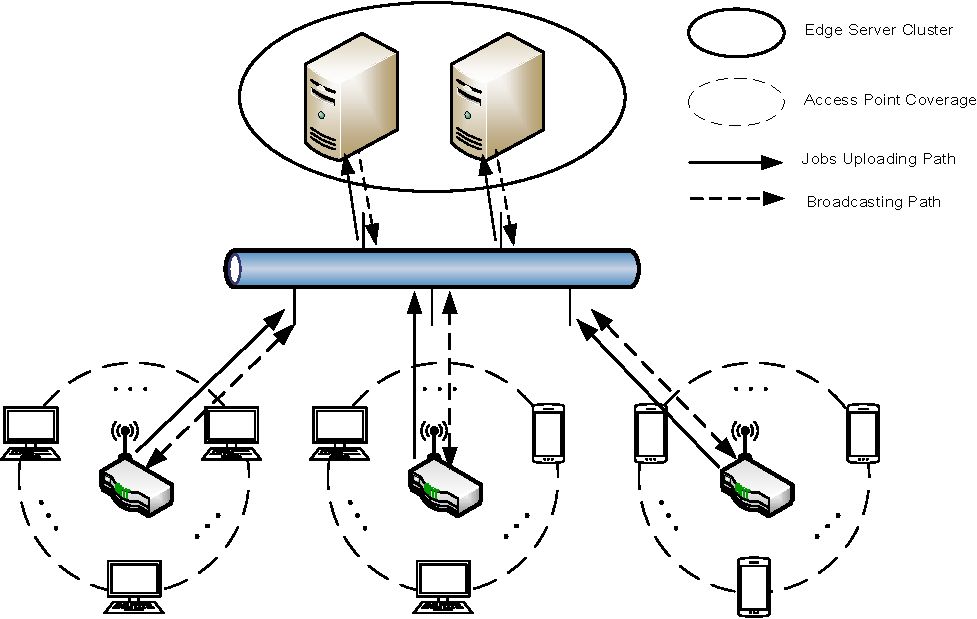
\includegraphics[width=0.80\textwidth]{system-model.pdf}
    \caption{The Illustration of MEC System Model}
    \label{fig:system}
\end{figure*}

%NOTE: [job space support and arrival process]
The time axis is organized by time slots.
The job arrivals in each time slot on each AP are modelled via independent Bernoulli distributions.
Specifically, the arrivals of the $j$-th job type at the $k$-th AP in different time slots are independent and identically distributed (i.i.d) Bernoulli random variables, and the arrival probability is denoted as $\lambda_{k,j}$ ($\forall k\in\apSet, j\in\jSpace$).
Let $A_{k,j}(t) \in \set{0,1}$ represents the event of job arrival, where $A_{k,j}(t)=1$ means one job of the $j$-th job type arrives on the $k$-th at the $t$-th time slot, and $A_{k,j}(t)=0$ means other wise.
Hence,
\begin{align}
    \Pr\{ A_{k,j}(t) = 1 \} = \lambda_{k,j}, \forall t,k\in\apSet,j\in\jSpace
\end{align}

%NOTE: [uploading process]
Each AP then immediately dispatches each type of received jobs to one edge server.
Different types of jobs may have different distributions on the input data size.
Moreover, due to the random traffic in the network, the job uploading from one AP to one edge server consumes a random number of time slots.
It is assumed that the distributions of uploading time are independent between any two uploading jobs.
Hence, we denote $\mathcal{U}_{k,m,j}$ as the uploading time for the $j$-th job type uploading from the $k$-th AP to the $m$-th edge server following some distribution with support $\set{1, \dots, \Xi}$, where $\Xi$ denotes the maximum uploading time ($\forall k\in\apSet, m\in\esSet, j\in\jSpace$).
In practice, the distribution of uploading latency may not be known to the APs or edge servers in advance.

%NOTE: [processing process]
There are $J$ virtual machines (VMs) running parallel on each edge server for the computation of $J$ job types, respectively.
For each job type, the uploaded jobs are computed in a First-Come-First-Serve (FCFS) manner.
Hence, a processing queue with maximum $L_{max}$ jobs is established for each VM.
The arrival jobs will be discarded when the processing queue is full.
Furthermore, we adopt the \emph{unrelated machines assumption} in \cite{tan-online} for job processing on edge servers.
Specifically, it is assumed that the computation time of different job types on different edge servers follows the memory-less Geometric distribution (with the unit of time slot) with different expectations.
Let $C_{m,j} \sim \mathbb{G}(1/c_{m,j})$ be the computation time distribution of the $j$-th job type on the $m$-th edge server, where $c_{m,j}$ is the expectation.
Hence, the probability mass function (PMF) of $C_{m,j}$ is given by:
\begin{align}
    f_{m,j}(k) \define (1-\frac{1}{c_{m,j}})^{k-1} \frac{1}{c_{m,j}}.
\end{align}
%----------------------------------------------------------------------------------------%

\subsection{Periodic Broadcast of State Information}
In order to facilitate cooperative dispatching for the APs, it is assumed that all the APs and edge servers will broadcast their \emph{local state information} (LSI) every $t_B$ time slots.
% as depicted in Fig.\ref{fig:brd-timeline}.
We shall refer to every $t_B$ time slots as a broadcast interval.
At the beginning of each broadcast interval (say the $t$-th broadcast interval), the LSI for AP and edge server is defined as follows, respectively.

%NOTE: State and Broadcast Information for AP
\begin{definition}[Local State Information of AP]
    One AP shall maintain LSI about the number of jobs in uploading, and the dispatching choice on edge servers for each job type.
    Specifically, at the $n$-th time slot in the $t$-th interval, the number of the $j$-th type job being uploaded $\xi$ time slots ago from the $k$-th AP to the $m$-th edge server is denoted as
    $R^{(k)}_{m,j,\xi}({t,n})$;
    at the $t$-th broadcast time slot, the dispatching choice of the $k$-th AP for proceesing of the $j$-th job type is denoted as
    $\omega_{k,j}(t) \in \esSet_{k}$ ($\forall k\in\apSet, m\in\esSet, j\in\jSpace, \xi\in(0,\Xi]$).
    
    Hence, the LSI of the $k$-th AP at the $t$-th broadcast is given as follows.
    \begin{align}
        \mathcal{R}_{k}(t) \define \set{\vec{R}^{(k)}_{m,j}(t,0), \set{\omega_{k,j}(t)|\forall j\in\jSpace} | \forall m\in\esSet_{k}, j\in\jSpace},
    \end{align}
    where
    $\vec{R}^{(k)}_{m,j}(t,0) \define ( R^{(k)}_{m,j,0}(t,0), \dots, R^{(k)}_{m,j,\Xi}(t,0) )$
    denotes the vector of random variables.
\end{definition}

%NOTE: State and Broadcast Information for ES
\begin{definition}[Local State Information of Edge Servers]
    One edge server shall maintain LSI about the computing queue status for each VM.
    Specifically, at the $n$ time slot in the $t$-th interval, the $m$-th edge server have $Q_{m,j}({t,n})$ denote the pending number of the $j$-th type job ($\forall m\in\esSet, j\in\jSpace$).

    Hence, the LSI of the $m$-th edge server at the $t$-th broadcast is defined as follows.
    \begin{align}
        \mathcal{Q}_{m}(t) \define \set{Q_{m,j}(t, 0) | \forall j\in\jSpace}.
    \end{align}
\end{definition}

We refer to \emph{global state information} (GSI) as the composition of all the broadcast information from all APs and edge servers in one broadcast and the definition is given as follows.
\begin{definition}[Global State Information]
    \begin{align}
        \Obsv^{\dagger}(t) \define
            \Brace{
                \mathcal{R}_{k}(t), \mathcal{Q}_{m}(t) | \forall k\in\apSet, m\in\esSet
            },
    \end{align}
    which is composed of all the broadcast information from all APs and edge servers at the $t$-th broadcast time slot.
\end{definition}

\begin{figure}[tp]
    \centering
    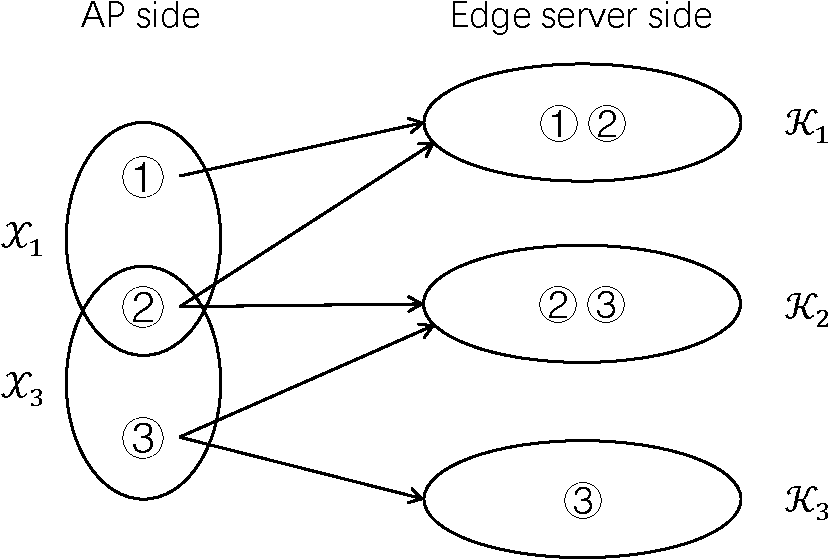
\includegraphics[width=0.45\textwidth]{images/conflict.pdf}
    \caption{The Example Illustration of Conflict Set and Partial Broadcast Information}
    \label{fig:conflict}
\end{figure}

%NOTE: Conflict of AP set and partial information definition
\comments{
    As the edge computing network resides in MAN, the propagation delay of LSI in such extensive network is not negligible.
    Thus for the $k$-th AP ($\forall k\in\apSet$), the reception latency of the LSI from the edge servers out of its \emph{candidate server set} $\esSet_{k}$ may be not acceptable.
    To alleviate the impact of information reception latency on decision making, we should leverage the definition of \emph{candidate server set} and \emph{candidate AP set}, and only use partial information from GSI for decision making for each AP.
}
Hence, we first define the \emph{conflict AP set} as follows.
\begin{definition}[Conflict AP Set]
    \begin{align}
        \ccSet_{k} \define \bigcup_{m\in\esSet_{k}} \apSet_{m}.
        % \ccSet_{k} \define \set{\forall k' \neq k\in\apSet|\esSet_{k'} \cap \esSet_{k} \neq \emptyset}
    \end{align}
    The \emph{conflict AP set} indicates that the subset of APs whose LSI could affect the decision making for the $k$-th AP.
\end{definition}

\begin{figure*}[t]
    \centering
    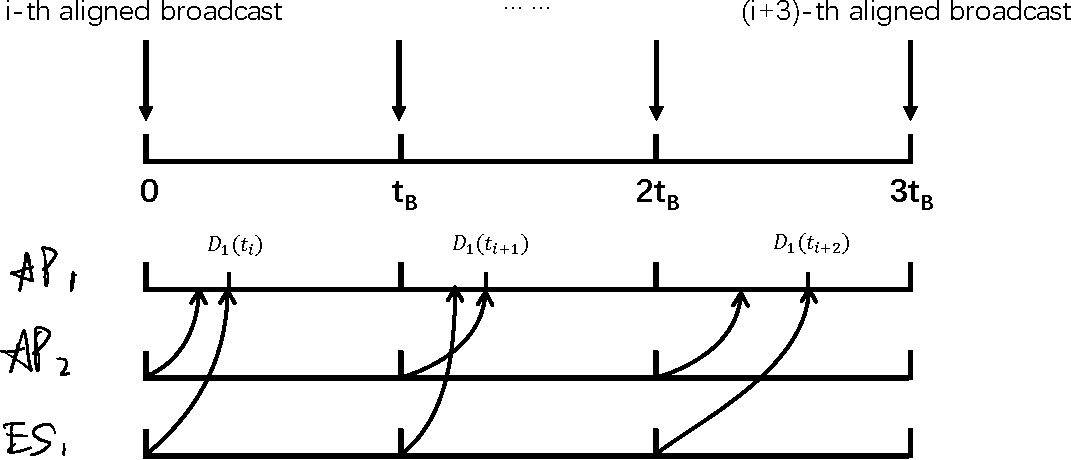
\includegraphics[width=0.80\textwidth]{brd-timeline.pdf}
    \caption{The timeline illustration of reception of OSI for the $1^{st}$ AP with the system setting in Fig.\ref{fig:conflict}.}
    \label{fig:brd-timeline}
\end{figure*}

It is assumed that each AP only collect the LSI from the APs in its \emph{conflict AP set} and edge servers from its \emph{candidate server set}.
For a simple example given in Fig.\ref{fig:conflict}, the $1^{st}$ AP only receives LSI from the $2^{nd}$ AP who is in its \emph{conflict AP set}, and LSI from the $1^{st}$ edge server who is in its \emph{candidate server set}.
Hence, we refer to the partial state information as \emph{observed state information} (OSI) and the definition is given as follows.
\begin{definition}[Observed State Information]
    The OSI for the $k$-th AP ($\forall k\in\apSet$) is defined as:
    \begin{align}
        \Obsv_{k} &= \set{\mathcal{R}_{k'} | \forall k'\in\ccSet_{k}}
                        \cup \set{\mathcal{Q}_{m} | \forall m\in\esSet_{k}}.
    \end{align}
\end{definition}

It is assumed that the $k$-th AP is able to collect its OSI $D_{k}(t)$ time slots later after the $t$-th broadcast time slot, where $D_{k}(t)$ is a random variable follows some distribution.
We refer to $D_{k}(t)$ as the \brlatency of the $k$-th AP for the $t$-th broadcast, which is upper bounded by the broadcast interval length $t_B$, i.e. $t_B > \hat{D}_{k}$ where $\hat{D}_{k}$ is the upper bound for $D_{k}(t)$ ($\forall k\in\apSet$).
Hence, $D_{k}(t)$ follows some distribution with support $\set{1,\dots,t_B}$, i.e. the broadcast interval $t_B$ is set that the $k$-th AP ($\forall k\in\apSet$) could receive the complete OSI before the start of next broadcast interval.

One AP shall update its dispatching decision immediately after the reception of its OSI.
An example is given to elaborate the decision as follows.
\begin{example}
    According to Fig.\ref{fig:brd-timeline}, we only consider the decisions update for the $1^{st}$ AP.
    In the first broadcast interval, it updates its dispatching decisions for all the job type $D_{1}(t)$ time slots later after the $t$-th broadcast, which is denoted as $\set{\omega_{1,j}(t+1) | \forall j\in\jSpace}$.
    At the start of the second broadcast interval, it will firstly keep the the previous decisions unchanged, and then updates the decisions immediately $D_{1}(t+1)$ time slots later which is denoted as $\set{\omega_{1,j}(t+2) | \forall j\in\jSpace}$.
    And then it repeats the process for the remaining of the time.
\end{example}

%----------------------------------------------------------------------------------------%

%----------------------------------------------------------------------------------------%
    \section{POMDP-based Problem Formulation}
\label{sec:formulation}
%----------------------------------------------------------------------------------------%
In this section, we formulate the optimization of job dispatching at all APs as a Markov decision process (MDP) problem.
Since each AP update the job dispatching actions according to OSI instead of GSI, the MDP problem is a partially observable MDP (POMDP).
Specifically, the individual dispatching policy of one AP, the system dispatching policy, and the cost function are first defined below.

\begin{definition}[Dispatching Policy]
    The individual policy of the $k$-th AP, denoted as $\Omega_{k}$ ($\forall k \in\apSet$), maps from its OSI $\Stat_{k}$ and its \brlatency~$\mathcal{D}_{k}$ to the dispatching action for each job type, i.e.,
    \begin{align}
        \Omega_{k} \Paren{ \Stat_{k}(t), \mathcal{D}_{k}(t) }
        &\define \mathcal{A}_{k}(t+1)
        \nonumber\\
        &= \Brace{
            \omega_{k,j}(t+1) \Big| \forall j\in\jSpace
        }.
        \label{def:action}
    \end{align}

    The aggregation of individual policy of all APs is referred to as the system dispatching policy $\Policy$.
    Thus,
    {\small
    \begin{align}
        \Policy\Paren{ \Stat(t), \Delay(t) } \define \Brace{
            \Omega_{1}(\Stat_{1}(t), \mathcal{D}_{1}(t)), \dots, \Omega_{K}(\Stat_{K}(t),\mathcal{D}_{K}(t))
        },
    \end{align}
    }
    where $\Delay(t) \define \set{ \mathcal{D}_{1}(t), \dots, \mathcal{D}_{K}(t) }$.
\end{definition}

% In the edge computing system, each AP individually performs job dispatching decision, and coordinates in a fully cooperative manner by sharing the same utility function.
% We propose the job dispatching optimization problem with the target to minimize the \emph{average response time}, which consists of the uploading time, waiting time and processing time, of all offloaded jobs in MEC system.
According to the Little's law \cite{Little1961}, the average response time per job, counting the number of broadcast intervals from job arrival to the accomplishment of computation, is proportional to the number of jobs in the system, given the job arrival rates at all the APs.
Hence, we define the cost function per broadcast interval as follows.

\begin{definition}[Cost Function per Broadcast Interval]
    The cost function of the $t$-th broadcast interval with GSI $\Stat(t)$ is defined as
    {\small
    \begin{align}
        g\Paren{\Stat(t)} \define
            \sum_{m\in\esSet,j\in\jSpace}
            \Brace{&
                \sum_{k\in\apSet} \Inorm{\vec{R}^{(k)}_{m,j}(t,0)} + Q_{m,j}(t,0)
                \nonumber\\
                &~~~~~+ \beta \cdot I[Q_{m,j}(t,0)=L_{max}]
            },
    \end{align}
    }where $\Inorm{\vec{x}}$ denotes the $L^1$-norm of the vector $\vec{x}$, and $\beta$ is the weight of overflow penalty.
\end{definition}

Since the job dispatching in one broadcast interval will affect the GSI of the following broadcast intervals, we should consider the joint minimization of the costs of all the broadcast intervals.
Specifically, we consider the following discounted sum of the costs of all the broadcast intervals as the system objective.
{\small
\begin{align}
    &\bar{G}(\Stat, \Policy) \define
    \lim_{T \to \infty} \mathbb{E}^{\Policy}_{\set{\Stat(t)|\forall t}}
    \Bracket{
        \sum_{t=1}^{T} \gamma^{t-1} g\Paren{\Stat(t)} \Big| \Stat(1)
    },
\end{align}
}where $\mathbb{E}^{\Policy}_{\set{\Stat(t)|\forall t}}[\cdot]$ denotes the expectation with respect to all possible system state in the future given scheduling policy $\Policy$, and $\gamma \in (0,1)$ is the discount factor.
Hence, the optimization of job dispatching policy can be formulated as the following minimization problem.
\begin{align}
    \textbf{P1:}~
    \min_{\Policy} \bar{G}(\Stat, \Policy).
\end{align}

If the GSI $\Stat(t)$ and \brlatency~$\Delay(t)$ are known to all the APs, the MDP in problem P1 can be solved via the following Bellman's equations as in \cite{sutton1998}.
\begin{align}
    &V\Paren{\Stat(t)} =g\Paren{\Stat(t)}
        + \gamma\mathbb{E}_{\Delay}\bigg\{
            \min_{\Policy(\Stat(t),\Delay(t))}
            \nonumber\\
            &\sum_{\Stat(t+1)} \Pr \Big\{ 
                \Stat(t+1) \Big| \Stat(t), \Policy(\Stat(t), \Delay(t)) \Big\} \cdot V\Big(\Stat(t+1)\Big)
            \bigg\},
    \label{eqn:sp_0}
\end{align}
where the value function $V(\Stat(t))$ of the optimal policy $\Policy^{*}$ (if GSI and \brlatency~are known to all the APs) is defined as follows.
\begin{align}
    &V\Paren{\Stat(t)} \define
    \lim_{T\to\infty} 
    \mathbb{E}^{\Policy^*}_{\set{\Stat(t)|\forall t}, \Delay} \Bracket{
        \sum_{t=1}^{T} \gamma^{t-1} g\Big( \Stat(t) \Big) \Big| \Stat(1)
    }.
    \label{eqn:val_f}
\end{align}
Moreover, the optimal policy $\Omega^{*}$ can be obtained by solving the right-hand-side (RHS) of the above Bellman's equations.

However, it is infeasible to solve the above Bellman's equations in our problem {and achieve the performance of $\Policy^*$ in our problem.}
This is because each AP (say the $k$-th AP) only has the knowledge of its own OSI $\Stat_{k}(t)$ and local \brlatency~$\mathcal{D}_{k}(t)$.
Thus, problem P1 is actually a POMDP.
The general solution of POMDP is of huge complexity {as all the historical system states should be involved in the current system state} \cite{IJCAI03-NairR,IJCAI99-BoutilierC}.
In this paper, we shall propose a novel low-complexity solution framework based on an analytical approximation of the value function $V(\cdot)$ and alternative actions update, where distributed job dispatching via the Bellman's equations becomes feasible even with OSI and local signaling latency.
%----------------------------------------------------------------------------------------%


    \section{Decentralized Algorithm with Partial Information}
\label{sec:algorithm}
Generally speaking, the optimal policy could be obtained by solving the minimization problem on the right-hand-side of the above Bellman's equation. %Eqn. (\ref{eqn:sp_0}).
In our problem, however, the GSI is not available and the centralized agent design is impractical due to randomness of \brlatency.
On the other side, conventional value iteration algorithm is intractable due to the tremendous state space.
The number of system states and action space would grow exponentially with respect to the number of APs and edge servers.
In this section, we propose a low-complexity solution scheme where each AP updates its dispatching policy according to its OSI in an iterative manner.

\subsection{Low-Complexity Solution Framework}
In this part, we first introduce an approximation of value function.
Based on it, the optimization of the right-hand-side of the Bellman's equations in Eqn.(\ref{eqn:sp_0}) can be decoupled.
Specifically, the value function of the optimal policy is approximated as follows.
\begin{align}
    V\Paren{\Stat(t)} \approx&
        W^{\AP}_{\Baseline}\Paren{\mathcal{R}(t+1)} + W^{\ES}_{\Baseline}\Paren{\mathcal{Q}(t+1)}
    \nonumber\\
    =& \sum_{j\in\jSpace}\sum_{k\in\apSet}\sum_{m\in\esSet} \Bracket{
        \sum_{i=0}^{\infty} \gamma^{i+1} \Inorm{ \vecG{R}^{(k)}_{m,j}(t+i+1) }
    }
    \nonumber\\
    & + \sum_{j\in\jSpace}\sum_{m\in\esSet} \Bracket{
        \sum_{i=0}^{\infty} \gamma^{i+1} Q_{m,j}(t+i+1)
    },
    \label{eqn:approx}
\end{align}
where $\Baseline$ denotes the following baseline policy.
\begin{definition}[Baseline Policy]
    \begin{align}
        \Baseline &\define \Bracket{ \Pi_{1}, \dots, \Pi_{K} }
        \\
        \Pi_{k} &\define \Brace{\pi_{k,j}\in\esSet|\forall j\in\jSpace}, \forall k\in\apSet
    \end{align}
    The baseline policy is chosen as fixed policy which is invariant of system state.
\end{definition}

However, with the approximate value function, it is still infeasible to solve the right-hand-side of the Bellman's equations.
On the one hand, the GSI is not available and each AP updates its policy independently from its corresponding OSI.
On the other hand, the centralized agent design is impractical due to randomness of \brlatency.

Hence, we propose a novel alternative policy update framework to address the issue of incomplete system state information.
Specifically, we first introduce the following periodic AP update sequence.
The APs shall update their polices iteratively based on OSI following the order of index of set $apSet$ and then repeat the procedure with the period $K$.
Based on it, we propose the following \emph{alternative dispatching policy}.
\begin{definition}[Alternative Dispatching Policy]
    \begin{align}
        \tilde{\Policy}\Paren{ k, \Stat(t), \Delay(t) } \define \Brace{
            \Omega_{k}( \Stat_{k}(t), \mathcal{D}_{k}(t) )
        },
    \end{align}
    where $k+1 \equiv t \pmod{K}, \forall t$.
\end{definition}
\begin{remark}
    In the \emph{alternative dispatching policy}, the index $k$ indicates that in the $t$-th interval only the $k$-th AP would update its policy while the other APs with policy fixed as broadcast in OSI of the $k$-th AP.
\end{remark}

Based on the proposed policy update framework, we further formulate the optimization problem as follows.
\begin{problem}[Alternative Optimization Problem]
    \begin{align}
        \min_{\tilde{\Policy}} \lim_{T\to\infty} \mathbb{E}_{\tilde{\Policy}} \Bracket{
            \sum_{t=1}^{T} \gamma^{(t-1)} g\Paren{
                \Stat(t), \tilde{\Policy}(\Stat(t), \Delay(t))
            } | \Stat(1)
        }.
    \end{align}
    \label{problem_2}
\end{problem}

\begin{lemma}
    With the \emph{alternative dispatching policy} framework, the approximated value function Eqn.(\ref{eqn:approx}) can be decoupled onto each AP in the following form.
    \begin{align}
        V_{k}(\Stat_{k}(t)) &\define W^{\AP}_{\Pi_{k}(t)}\Paren{\mathcal{R}(t+1)} + W^{\ES}_{\Pi_{k}(t)}\Paren{\mathcal{Q}(t+1)}
        \nonumber\\
        =& \sum_{j\in\jSpace}\sum_{k\in\ccSet_{k}}\sum_{m\in\esSet_{k}} \Bracket{
            \sum_{i=0}^{\infty} \gamma^{i+1} \Inorm{ \vecG{R}^{(k')}_{m,j}(t+i+1) }
        }
        \nonumber\\
        & + \sum_{j\in\jSpace}\sum_{m\in\esSet_{k}} \Bracket{
            \sum_{i=0}^{\infty} \gamma^{i+1} Q_{m,j}(t+i+1)
        },
    \end{align}
\end{lemma}
where
\begin{align}
    \Pi_{k}(t) = \set{\omega_{k,j}(t-1)|\forall j\in\jSpace}.
\end{align}

\subsection{The Decentralized Algorithm}
Then, we could propose the algorithm to solve the decentralized problem for each AP.
The decentralized problem for the AP is defined as follows.
% The optimization problem at right-hand side of approximate Bellman's Equation is given as follows.
\begin{problem}[Decentralized Approximated Optimization Problem for AP]
    For the $k$-th AP with baseline policy $\Pi_{k}(t)$:
    \begin{align}
        \min_{\Pi_{k}(t)} \mathbb{E}_{\set{ \Stat(t+1), \Pi_{k}(t) }} \Bracket{
            W^{\AP}_{\Pi_{k}(t)}\Paren{\mathcal{R}(t+1)} + W^{\ES}_{\Pi_{k}(t)}\Paren{\mathcal{Q}(t+1)}
        }.
        \label{eqn:partial}
    \end{align}
\end{problem}

The expected value function $W^{\AP}_{\Pi_{k}(t)}(\mathcal{R}(t+1))$ is easily obtained by calculating the following equation.
\begin{align}
    W^{\AP}_{\Pi_{k}(t)}\Paren{\mathcal{R}(t+1)} = \sum_{j\in\jSpace}&\sum_{k\in\ccSet_{k}}\sum_{m\in\esSet_{k}}
    \nonumber\\
    &\Inorm{
        \Paren{ 1 - \gamma ({\Gamma}^{(k)}_{m,j})^{N} }^{-1} \hat{\vecG{\Theta}}^{(k)}_{m,j}(t+1)
    }.
    \label{w_ap}
\end{align}
% where $\hat{\Gamma}^{(k)}_{m,j} \define (\Gamma^{(k)}_{m,j})^{N}$.

The expression for expected value function $W^{\ES}_{\Pi_{k}(t)}(\mathcal{Q}(t+1))$ is little more complex compared to Eqn.(\ref{w_ap}).
It is affected with both arrival process under dispatching policy and last queue state.
However, we notice that the arrival process would be stationary after the maximum uploading time under the stationary baseline policy and the relationship between APs and edge server could be decoupled.
\begin{align}
    W^{(k)}_{\Baseline(t)}\Paren{\mathcal{Q}(t+1)}
    =& \sum_{j\in\jSpace}\sum_{m\in\esSet_{k}}\sum_{i=0,\dots,\frac{\Xi}{T}} \gamma^{i} \mathbb{E}[ Q_{m,j}({t+i+1}) ]
    \nonumber\\
    &~~~~~~~~+ \gamma^{\frac{\Xi}{T}} \Paren{ \mat{I} - \gamma \hat{\mat{P}}_{m,j}(\tilde{\beta}_{m,j}) }^{-1} \vecG{\nu}({t+\frac{\Xi}{T}+1}) \vec{g}',
\end{align}
where the $i$-th element of vector $\vec{g}$ denotes the cost of server as $Q_{m,j}(t)$;
\begin{align}
    \hat{\mat{P}}_{m,j}(\tilde{\beta}_{m,j}) \define \prod_{n=0,\dots,N-1} \mat{P}_{m,j}(\tilde{\beta}_{m,j})
\end{align}
% the probability distribution of $Q_{m,j}({t+i+1})$ is denoted by $\vecG{\nu}({t+i+1})$ which is obtained by calculating equation Enq. (\ref{eqn_0}) - Eqn. (\ref{eqn_4}) ($\forall i=0,\dots,\frac{\Xi}{T}$);
where $\tilde{\beta}_{m,j}$ is the arrival distribution under baseline policy $\Pi(t)$ (on $m$-th ES with $j$-type job)
\begin{align}
    \tilde{\beta}_{m,j} &\define \sum_{k\in\apSet} \tilde{\lambda}^{(k)}_{m,j} \times \sum_{\xi=0,\dots,\Xi-1} \Pr\{ \xi<U_{k,m}\leq(\xi+1) \}
        \nonumber\\
    ~~~~&= \sum_{k\in\apSet} \tilde{\lambda}^{(k)}_{m,j}
\end{align}

The details of the procedure is elaborated as follows.
\begin{itemize}
    \item Choose the initial \emph{system dispatching policy} start with some heuristic policy.
    \item At the first broadcast time slot when $t=0$, the APs and edge servers in \emph{conflict AP set} and \emph{candidate server set}, respectively, of the $1$-st AP would broadcast their LSI (including the heuristic policies);
    \item The $1$-st AP would receive the OSI at the $D_1(1)$ time slots in the first broadcast interval, and then it updates its policy $\Omega_{1}(\Stat_{1}(1))$ by solving Eqn.(\ref{eqn:sp_0}) for the $1$-st AP.
    The $1$-st AP would keep with this policy until it receives the OSI again.
    \item At the second broadcast time slot when $t=1$, the OSI of the $2$-nd AP would be broadcast;
    the $1$-st AP would broadcast $\Omega_{1}(\Stat_{1}(1))$ if it's in the \emph{conflict AP set} of the $2$-nd AP;
    \item Similarly, in the $t$-th broadcast interval the AP indexed with $k' \equiv (t + 1)\mod{K}$ would receive the OSI $D_{k'}(t)$ time slots later, and then it updates its policy $\Omega_{k'}(t+1)$ by solving Eqn.(\ref{eqn:sp_0}) for the $k'$-th AP.
\end{itemize}

% \begin{lemma}
%     The optimized policy solved as $\Baseline(t)$ for next stage, is better than $\Baseline(t-1), \dots, \Baseline(1)$ when considering the \emph{approximated value function} defined above.
%     \\
%     Moreover, the performance of the series of the baseline policies is upper bounded by the optimal solution $\Policy^*$ when considering the original Bellman's equation.
%     $$
%         V_{\Omega^*}\Paren{\Stat(t)}
%         \leq W_{\tilde{\Policy}(t)}\Paren{\Stat(t)}
%         \leq W_{\tilde{\Policy}(t-1)}\Paren{\Stat(t)}
%     $$
% \end{lemma}
% \begin{proof}
    
% \end{proof}

%----------------------------------------------------------------------------------------%
\delete{v11}{
    % [\IF, \ENDIF], [\FOR, \TO, \ENDFOR], [\WHILE, \ENDWHILE], \STATE, \AND, \TRUE
    % \begin{algorithm}[H]
    %     \caption{Online Iterative Policy Improvement Algorithm}
    %     \begin{algorithmic}[1]
    %         \STATE $t = 0$
    %         \FOR{$t = 1,2,\dots$}
    %             \STATE Evaluate $\Omega_0$ in \textbf{P1} according to Eqn. (\ref{sp1})
    %             \FOR{$k \in \mathcal{K}$}
    %                 \STATE fix policy $\vec{\Omega}^{(k)}(t) \forall k' < k$
    %                 \STATE Evaluate $k$-th AP Local Policy $\tilde{\Omega}_k$ in \textbf{Pk} according to Eqn. (\ref{sp2})
    %             \ENDFOR
    %         \ENDFOR
    %     \end{algorithmic}
    % \end{algorithm}
}
%----------------------------------------------------------------------------------------%
    \section{Performance Evaluation}
\label{sec:evaluation}

\subsection{Experimental Setup}
\textbf{System Parameters Setup:}
We implement the system in a small scale setting where fully-accessible APs and edge servers are considered.
specifically, there are $K=8$ APs, $M=5$ edge servers, and $J=5$ type of jobs in the system corresponding to the manipulated data trace.
Each time slot is taken as $\tau = 0.05$ i.e. 50ms, and the broadcast interval is taken as $20$ time slots, i.e. $1$ second.
The maximum uploading time is set as $3$ times the broadcast interval, i.e. $\Xi = 3T$.
The distributions of arrival rate, uploading time and processing time are generated randomly.
Each queue for VMs on edge server is set with maximum queue length $L_{max}=20$.
% The arrival rate is taken as small probability with enough APs in the system, and correspondingly enough edge servers for the processing.
% Each queue on edge server with maximum 20 jobs because our algorithm is strong enough to predict the overflow to ensure a reliable system.

\textbf{Compared Algorithms:}
We compare the proposed algorithm with other three heuristic algorithms.
Compared Algorithm:
\begin{itemize}
    \item \textbf{Random Dispatching Policy}:
            randomly dispatch jobs to edge servers;
    \item \textbf{Local Selfish Algorithm (baseline policy)}:
            always choose the edge server with the minimum expected uploading time plus the expected processing time for each job type; this policy is also taken as the initial fixed policy of our proposed algorithm;
    \item \textbf{Local Queue-aware Greedy Algorithm}:
            always choose the edge server with the minimum expected uploading time, plus the expected queueing time based on the observation of stale queue state.
\end{itemize}
Specifically, we choose a heuristic selfish policy as the start and the definition is given as follows.
\begin{definition}[Selfish Policy]
    \begin{align}
        \Baseline &\define \Bracket{ \Pi_{1}, \dots, \Pi_{K} }
        \\
        \pi_{k,j} &\define \arg\min_{m} \mathbb{E}[U_{k,m,j}] + \mathbb{E}[C_{m,j}]
    \end{align} 
\end{definition}
%----------------------------------------------------------------------------------------%

\subsection{Performance Analysis}
    \subsubsection{Basic Performance}
    Here we measure some basic metrics concerning in edge computing system, compared with different algorithms.
    \begin{itemize}
        \item Bar graph: Cost v.s. Algorithms;
        \item Bar graph: JCT v.s. Algorithms;
        \item Bar graph: Total Departure Rate v.s. Algorithms. 
    \end{itemize}

    \subsection{Fine-grained Analysis}
    \begin{itemize}
        \item Timeline graph: our proposed algorithm is better than compared algorithms all the time in Fig.\ref{fig:general_timeline};
        \item CDF of Cost (with different algorithms);
        \item CDF of JCT (with different algorithms);
    \end{itemize}

    \subsubsection{Sensitivity Study}
    \begin{itemize}
        \item \textbf{Different number of APs.} (a.k.a arrival rate)
        \item \textbf{Uploading time domains/Processing time domains.}
        \item \textbf{Compared with different \brlatency.} Fig.\ref{fig:eval_delay}
        \item \textbf{Different $t_B$ setting.}
        \item \textbf{Different Penalty Factors.}
    \end{itemize}
    % CDF of \# of dropped jobs (over the queue limit); CDF of queue length;
%----------------------------------------------------------------------------------------%

\begin{figure*}[htp!]
    \centering
    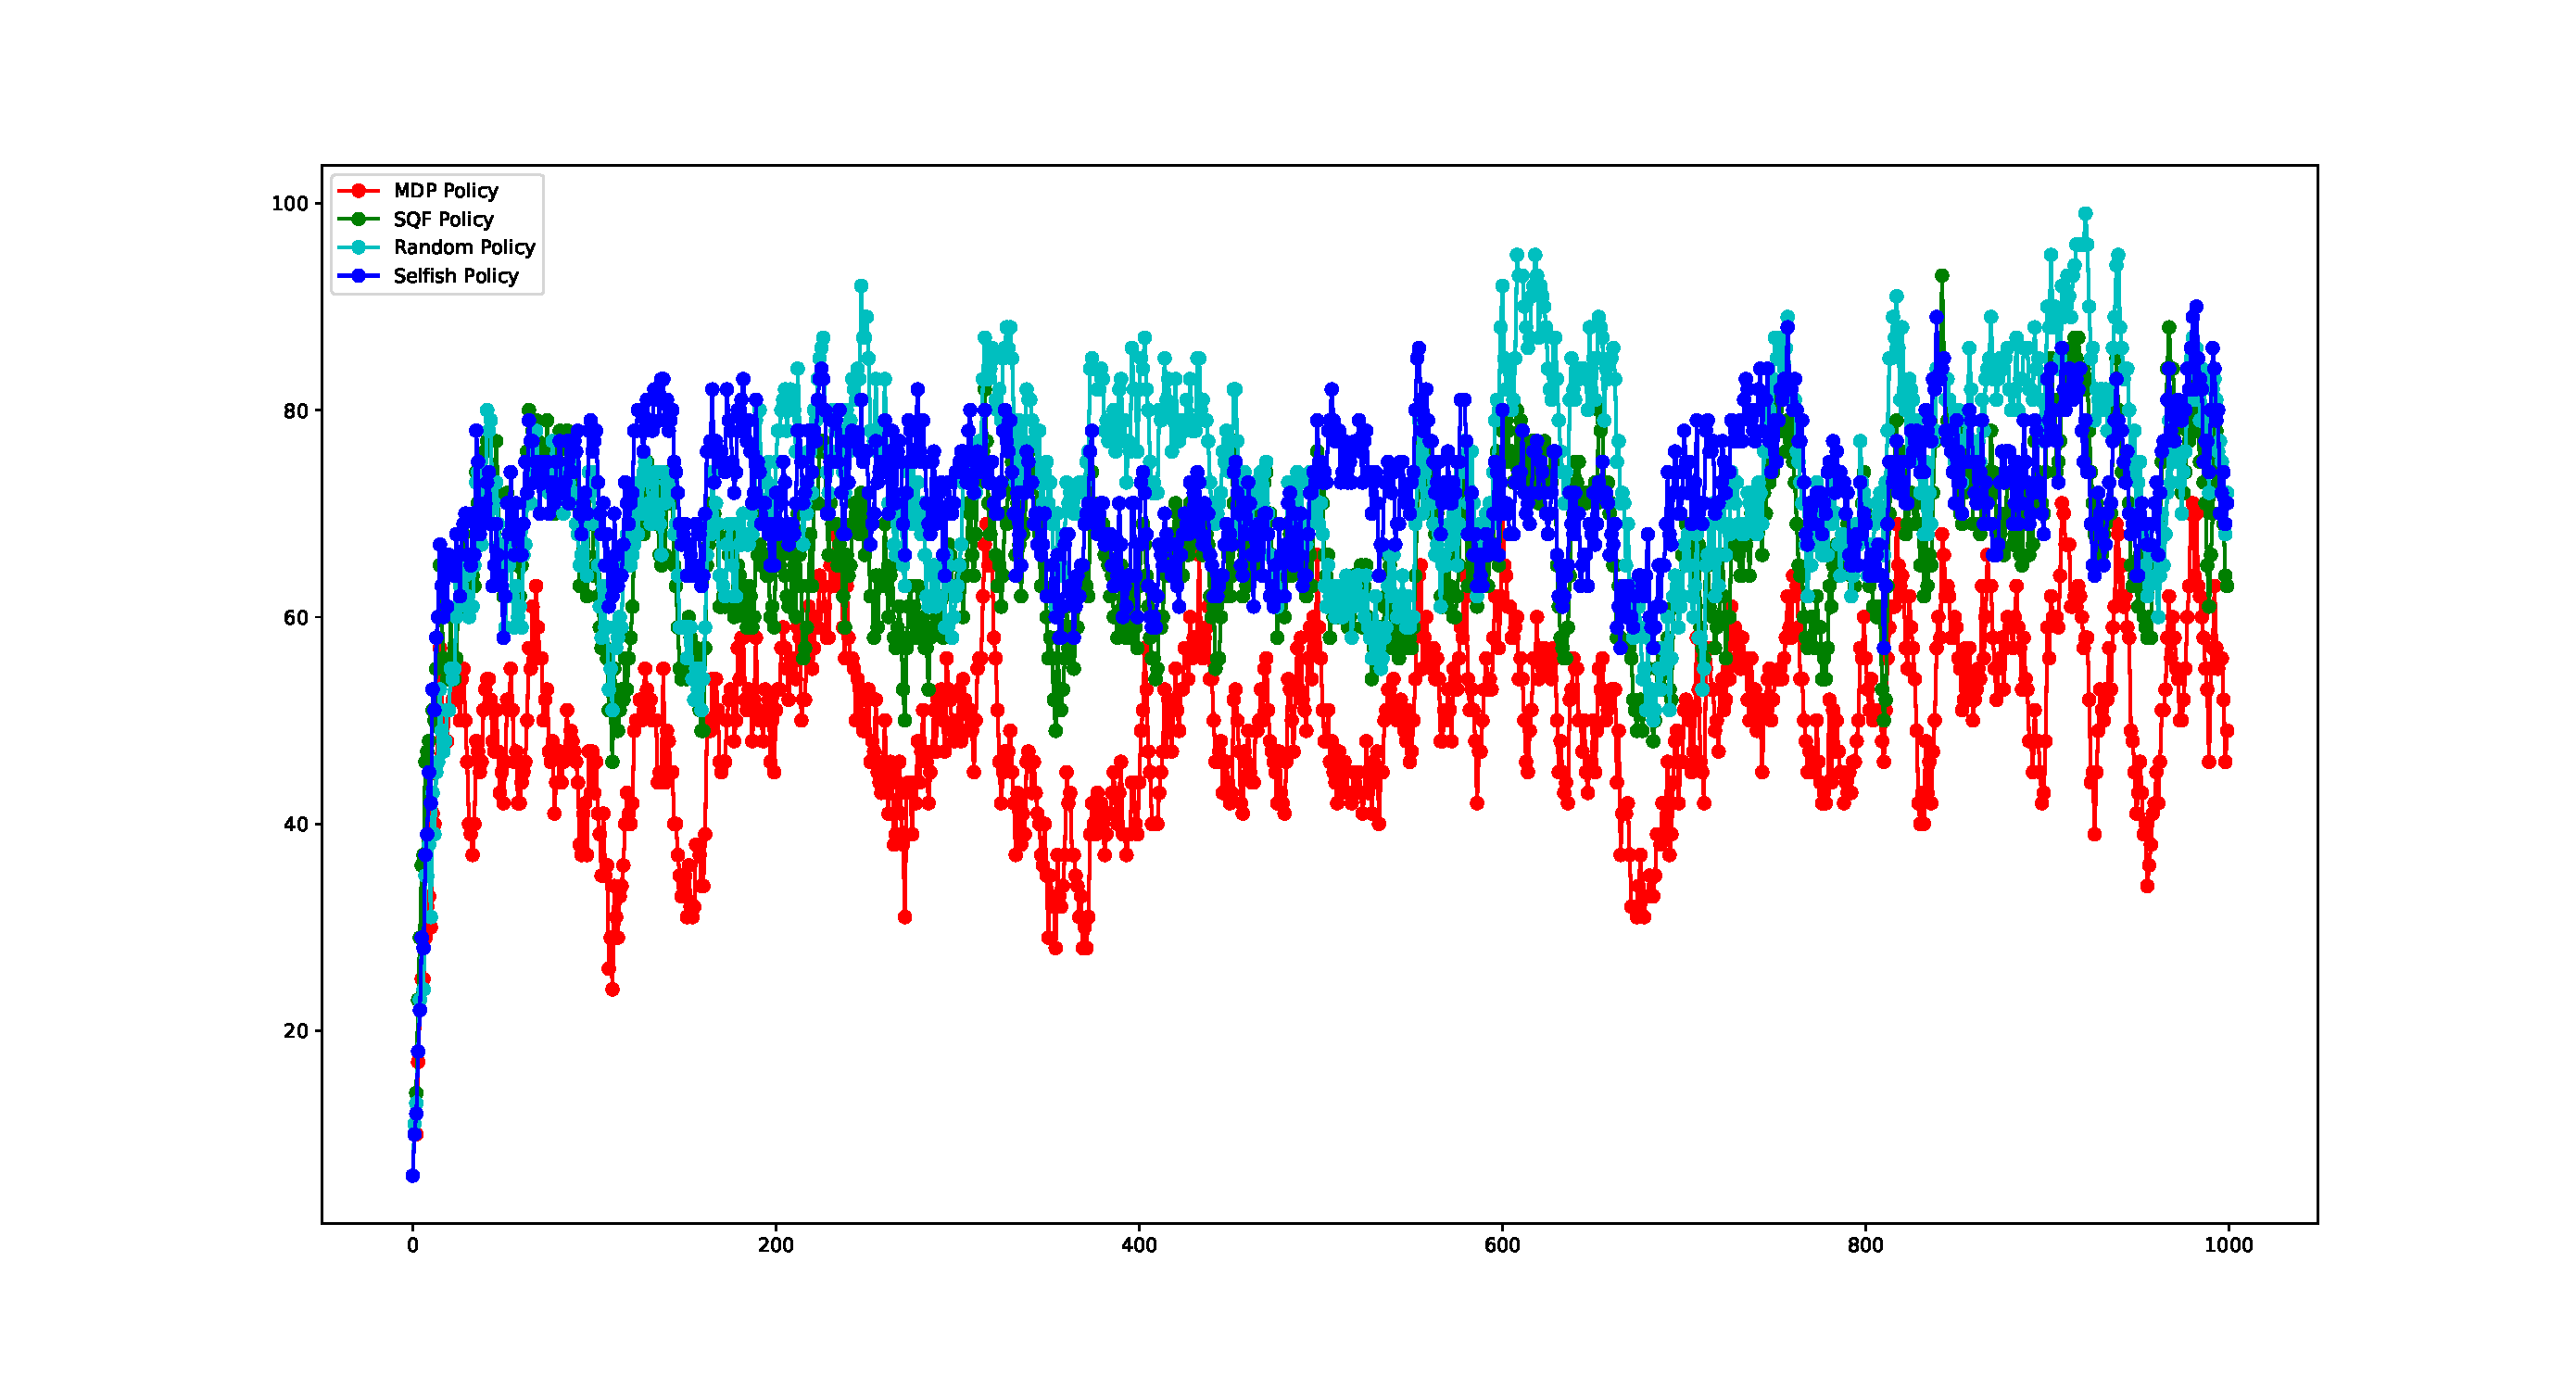
\includegraphics[width=0.80\textwidth]{images/Figure_1.pdf}
    \caption{Timeline illustration.}
    \label{fig:general_timeline}
\end{figure*}

\begin{figure*}[htp!]
    \centering
    \begin{tabular}{ccc}
        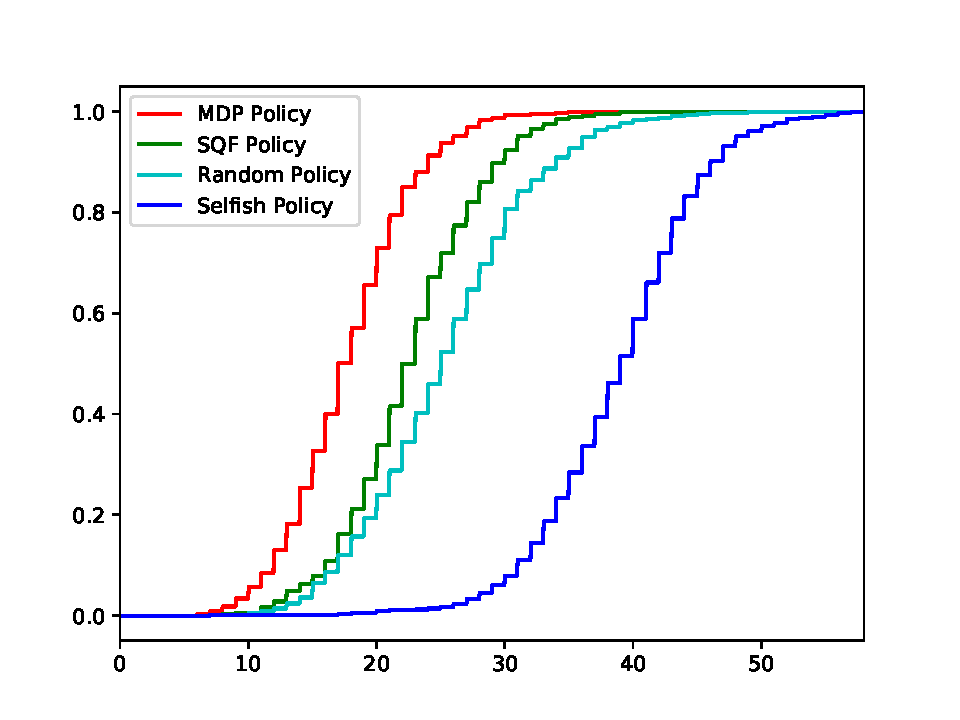
\includegraphics[width=0.30\textwidth]{images/535_LowPressure_NoDelay.pdf}&
        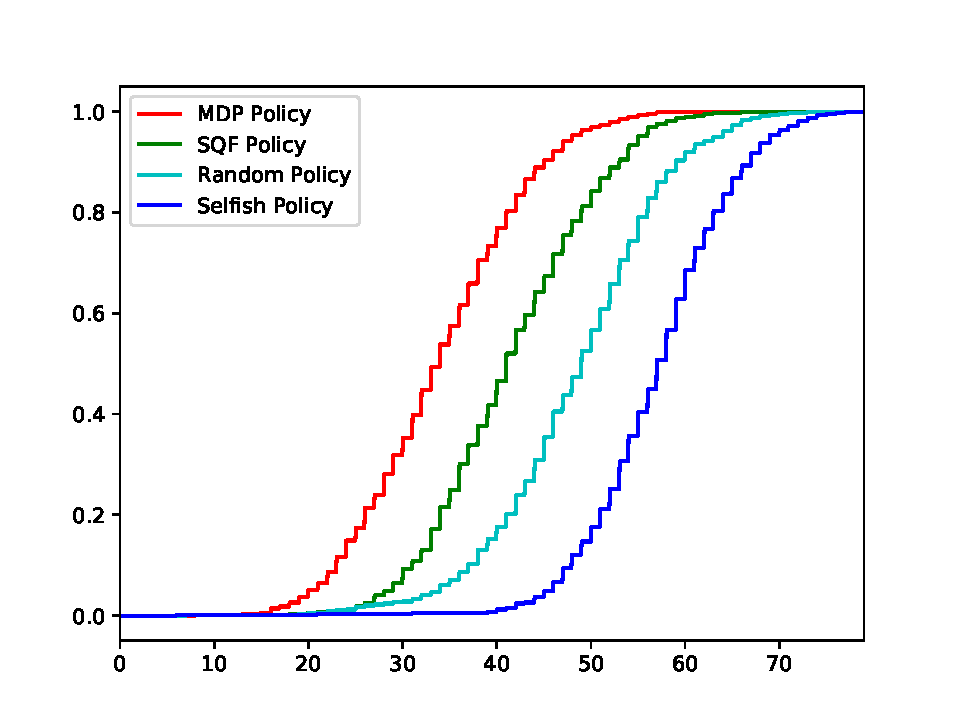
\includegraphics[width=0.30\textwidth]{images/535_LowPressure_LargeDelay_cdf.pdf}&
        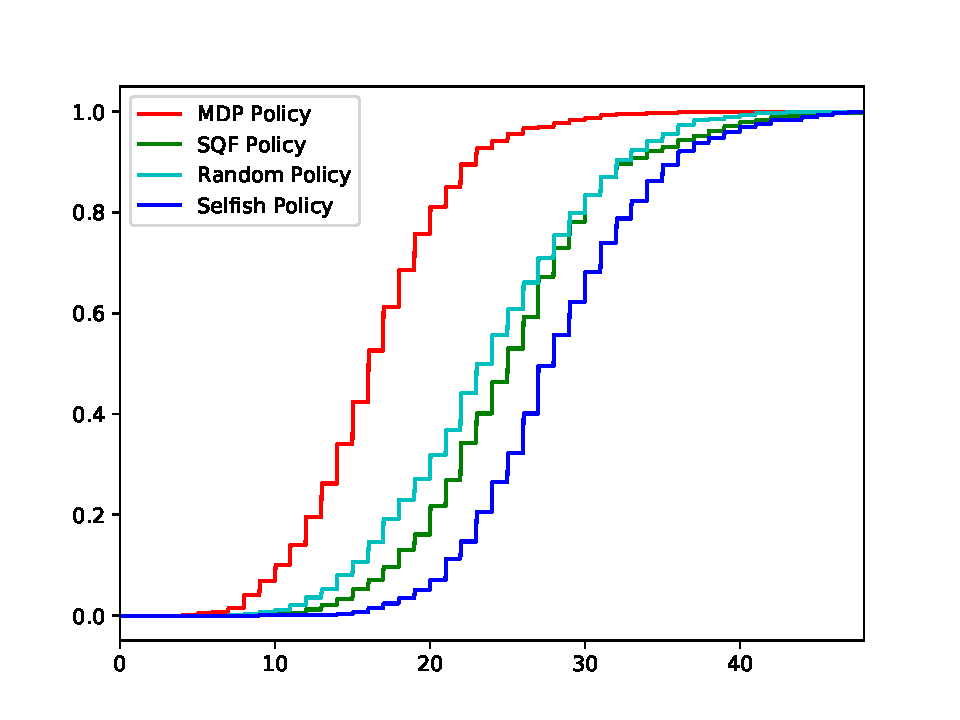
\includegraphics[width=0.30\textwidth]{images/535_LowPressure_FullDelay.pdf}
        \\
        {\small (a) No \brlatency} &
        {\small (b) Large \brlatency} &
        {\small (c) Whole-interval \brlatency}
    \end{tabular}
    \caption{Evaluation of Information Staleness Impact on Algorithm Robustness under Low Back Pressure.}
    \label{fig:eval_delay}
\end{figure*}

\delete{v12.2}{
    \textbf{Data Trace Extraction:}
    We use the Google data trace for cloud computing\needref{google-data-trace}.
    There is no broadcast latency, uploading time, and processing distribution information specified in the data trace.
    Hence, we extract and scale the arrival and processing time in the original data trace.
    And we manipulate the original data with random generated latency distribution.

    % [abandon, cause useless]
    \textbf{Estimation Error Analysis.}
    (If these graphs are not good, they are not going to appear on final draft.)
    \begin{itemize}
        \item Two curves, one for real cost against time slot, one for expected sampling cost against time intervals; (if the accumulate area within the latter one has little/bounded error with real cost, then it is okay and the correctness is support by simulation)
        \item 
    \end{itemize}
}
    \section{Conclusion}
\label{sec:conclusion}
In this paper, we consider a distributed and asynchronous job dispatching design in an edge computing network residing in a MAN with multiple APs and edge servers.
The APs and edge servers periodically broadcast their local state information to facilitate distributed dispatcher design.
Due to random transmission latency, the system information observed at different dispatchers are asynchronous.
We also consider a practical scenario that not all the state information can be observed by each AP.
We formulate the distributed optimization of job dispatching strategies at all the APs as a POMDP, whose minimization objective is a discount measurement of job delivery and computation time.
We propose a novel low-complexity distributed solution framework based on analytical approximation of value function and one-step policy iteration, where the complicated POMDP solution or value iteration is avoided and the analytical performance lower bound is derived.
The simulation results show that the proposed solution framework outperforms various benchmarks.
In the future work, we shall extend the proposed framework to a more general scenario where the knowledge on the distributions of signaling latency, uploading latency and computation time is absent.
The reinforcement learning would be integrated with the proposed solution framework to address the above issue.

    \clearpage
    \bibliographystyle{IEEEtrans}
    \bibliography{references/main.bib,references/related.bib}
\end{document}